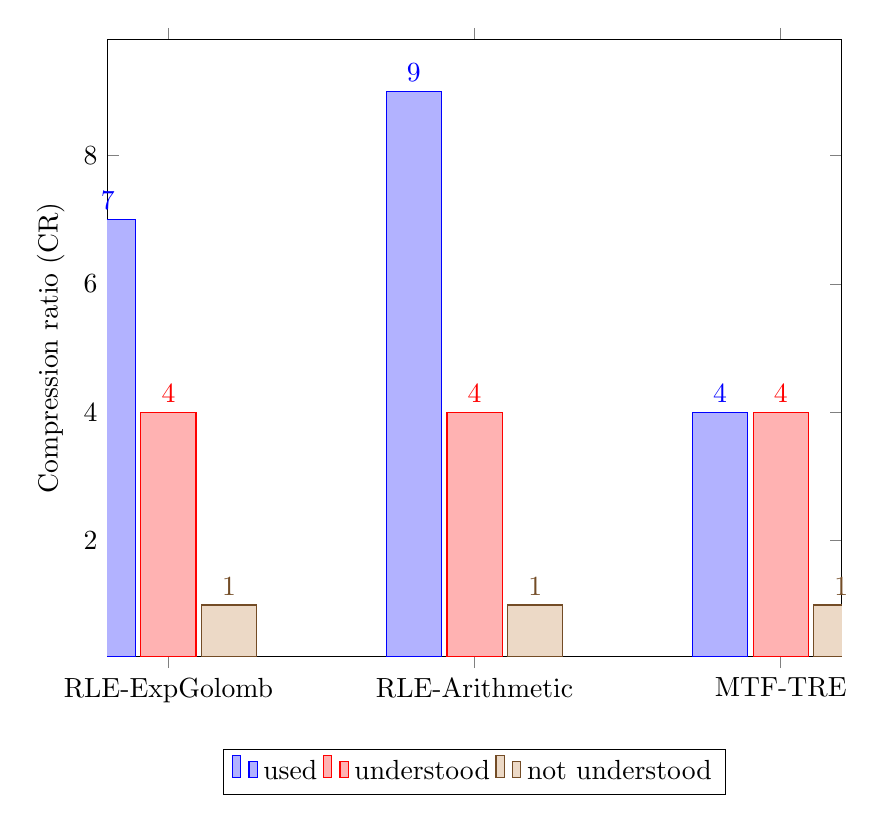
\begin{tikzpicture}
\begin{axis}[
	ybar,
	bar width = 0.7cm,
	width = .9\linewidth,
	enlargelimits=0.1,
	legend style={at={(0.5,-0.15)},
		anchor=north,legend columns=-1},
	ylabel={Compression ratio (CR)},
	symbolic x coords={RLE-ExpGolomb,RLE-Arithmetic,MTF-TRE},
	xtick=data,
	nodes near coords,
	nodes near coords align={vertical},
	]
	\addplot coordinates {(RLE-ExpGolomb,7) (RLE-Arithmetic,9) (MTF-TRE,4)};
	\addplot coordinates {(RLE-ExpGolomb,4) (RLE-Arithmetic,4) (MTF-TRE,4)};
	\addplot coordinates {(RLE-ExpGolomb,1) (RLE-Arithmetic,1) (MTF-TRE,1)};
	\legend{used,understood,not understood}
\end{axis}
\end{tikzpicture}